\chapter{Faster Queries using an Inverted Index}

\section{Task}
When using an search engine, the most important aspect is to be able to perform a search and get the results almost instantaneously. One way of doing this is by using an Inverted Index, which sorts the websites according to the words contained in each website. Hence when searching for a specific term, instead of going over every website, it will go over all the words instead and then provide the websites related to searched term. While building the Inverted Index can be system heavy, it is a one time operation that will allow the search engine to operate significantly faster.

\section{Basic Approach}
All the files regarding the classes mentioned on this chapter can be found on the folder src/main/java/searchengine.\\
The {\tt Index} was generalised into an interface to make it easy to test the different indices and switch between them. The following methods define the aforementioned {\tt Index} interface:
\begin{itemize}
    \item {\tt build} — Processes a list of websites into the data structure.
    \item {\tt lookup} — Given a query string, returns a list of all websites that contain such query.
    \item {\tt provideIndex} — Provides all websites in a given {\tt Index} as a collection. This specific method was added for the ranking algorithm and the testing of the index.
\end{itemize}
The inverted indices were then implemented using inheritance, since both the {\tt InvertedIndexHashMap} and {\tt InvertedIndexTreeMap} can be given exactly the same methods, being only difference their individual data structure.

\section{Technical Description}
As previously stated, a generalised {\tt Index} interface was created. Each of the classes below implements this interface, visualized in \ref{fig:Index:uml}.

\begin{figure}[!h]
    \centering
    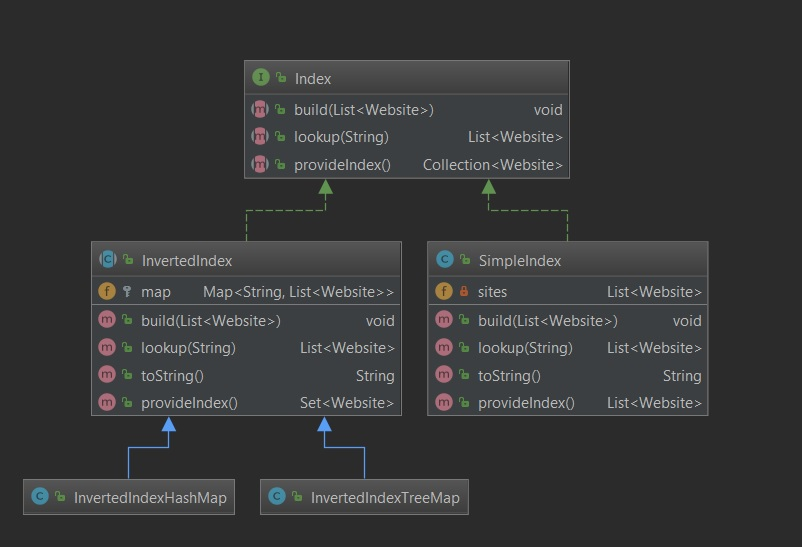
\includegraphics[width=\textwidth]{figures/Diagram_InvertedIndices}
    \caption{UML Diagram for the Software Architecture of Index data structures.}
    \label{fig:Index:uml}
\end{figure}

\subsection{{\tt SimpleIndex}}
The provided default way of indexing data was called {\tt SimpleIndex}. This solution is implemented looping through every word of every website, storing the matching website that matched the given query on an {\tt ArrayList<Website>}.\\

\subsection{{\tt InvertedIndex}}
The second (and improved) approach to index the data was to use an {\tt InvertedIndex}. As the name implies, here the relationship between a website and its words is inverted, meaning that each word knows to which sites it belongs to. In Java terms, {\tt Map}s are used where every word is a {\tt Key} with and associated {\tt Value}, which consists of an {\tt ArrayList<Website>}.\\
Since it did not make sense to create instances of {\tt InvertedIndex}, this class was made {\tt abstract} and, since it implemented methods of the {\tt Index} interface, it implements it.

\subsubsection{{\tt InvertedIndexTreeMap}}
This class {\tt extends InvertedIndex}.\\
The underlying data structure of the {\tt TreeMap} is a Red-Black tree based {\tt NavigableMap} implementation, sorted either by the natural ordering of its keys or by a {\tt Comparator}. {\tt TreeMap} provides \textit{guaranteed log(n) time} performance for the operations \textbf{containsKey}, \textbf{get}, \textbf{put}, \textbf{remove}.\cite{oracle:treemap} {\tt TreeMap} uses only the amount of memory needed to hold it's items, therefore this solution is suited when it is not known how many items have to be sorted in memory and there are memory limitations. Solutions is also suited when the order in which items have been stored is important and O(log n) search time is acceptable.\cite{baeldung:HashTreeCompared}

\subsubsection{{\tt InvertedIndexHashMap}}
This class {\tt extends InvertedIndex}.\\
The underlying data structure of the {\tt HashMap} is a hash table based implementation. This implementation provides \textit{constant-time} performance for the basic operations such as \textbf{get} and \textbf{put}.\cite{oracle:hashmap} However this is true under assumption that there are not too many collisions. This is because this {\tt Map} implementation acts as a basket hash table and when buckets get too large, they get transformed into tree nodes, similar to those of {\tt TreeMap}. \cite{baeldung:HashTreeCompared} Some of the downsides of building the HashMap are that it requires more memory than it is necessary to hold its data and when a HashMap becomes full, it gets resized and rehashed, which is costly.\cite{baeldung:HashTreeCompared}

\section{Benchmarking}
In order to choose one of the implementations, for the search engine, the benchmark test was performed to gain empirical data of the performance of each of the implementations. For the benchmark test, JMH (a Java harness for building, running, and analysing nano/micro/milli/macro benchmarks) was used. {OpenJDK:jmh} The benchmark test was carried out using 20 words (random nouns, verbs, adjectives and conjunctions), which were looked-up using the three different {\tt Index} implementations and in three different size databases: {\tt enwiki-tiny}, {\tt enwiki-small}, {\tt enwiki-medium}. JMH then provides information about an average Score, measured in nanoseconds per operation, whose results of which can be found in table \ref{table:result}\\
During the benchmark it was assured that the test environment is as similar as possible among the different trials, meaning that all tests were performed on the same machine and no other applications running on the background.
% Please add the following required packages to your document preamble:
% \usepackage{multirow}

\begin{table}[!h]
    \centering
    \caption{\textbf{Benchmark Scores. Each score is an average in ns/op}}
    \begin{tabular}{|l|r|r|r|l}
        \cline{1-4}
        \multicolumn{1}{|c|}{\multirow{2}{*}{\textbf{Data set}}} & \multicolumn{1}{c|}{\multirow{2}{*}{\textbf{Simple Index}}} & \multicolumn{2}{c|}{\textbf{Inverted Index}}                                  &  \\ \cline{3-4}
        \multicolumn{1}{|c|}{}                                   & \multicolumn{1}{c|}{}                                       & \multicolumn{1}{c|}{\textbf{HashMap}} & \multicolumn{1}{c|}{\textbf{TreeMap}} &  \\ \cline{1-4}
        enwiki-tiny                                              & 18 944,884                                                  & 1 052,067                             & 1 591,311                             &  \\ \cline{1-4}
        enwiki-small                                             & 8 819 338,592                                               & 1 883,776                             & 3 622,582                             &  \\ \cline{1-4}
        enwiki-medium                                            & 233 498 546,571                                             & 27 451,020                            & 30 176,993                            &  \\ \cline{1-4}
    \end{tabular}
    \label{table:result}
\end{table}
% Jonas' table, just in case.
% \begin{table}[!htbp]
%     \caption{\textbf{Benchmark Scores. Each score is an average in ns/op}}
%     \begin{tabular}{|p{75pt}|p{75pt}|p{75pt}|p{75pt}|}
%         \hline
%         \textbf{Data set} & \textbf{Simple Index} & \textbf{IE: HashMap} & \textbf{IE: TreeMap} \\ \hline
%         enwiki-tiny & 18 944,884 & 1 052,067 & 1 591,311 \\ \hline
%         enwiki-small & 8 819 338,592 & 1 883,776 & 3 622,582 \\ \hline
%         enwiki-medium & 233 498 546,571 & 27 451,020 & 30 176,993 \\ \hline
%     \end{tabular}
%     \label{table:result}
% \end{table}

The benchmark results shows that the {\tt SimpleIndex} is significantly slower than both of the {\tt InvertedIndex} implementations: 233 498 546,571 ns/op versus 27 451,020 ns/op for the {\tt InvertedIndexHashMap} and 30 176,993 ns/op for the {\tt InvertedIndexTreeMap} using the {\tt enwiki-medium} dataset.
In order to describe the results, let the number of websites be $m$ and words be $n$.
The difference in performance can be explained as follows:\\
When the {\tt SimpleIndex} is looking up the search word, it looks though all the sites, which takes \textit{O(m)} time, and for each site it looks through all the words which takes \textit{O(n)} time, therefore total search time is \textit{O($m\cdot n$)}. The two other methods provide faster performance time. {\tt InvertedIndexTreeMap} provides a \textit{guaranteed} performance of \textit{O(log(n))}. {\tt InvertedIndexTreeMap} provides best-case performance of constant time \textit{O(1)} and the worst-case performance of \textit{O(log(n))} time (since Java 8). Worst-case performance occurs when the hash function is not implemented correctly and values are distributed poorly in buckets, leading to high hash collision.\\
%$2 \cdot log(n) + occ$\
There are several considerations when choosing the implementation for storing the data for the Search Engine.\\
{\tt HashMap} seems to be better fit than a {\tt TreeMap} for our search Engine implementation, because in this case the order of data is not important whereas the performance looking up the websites corresponding the search word is. The {\tt HashMap} can be expected to perform in constant time which is better than {\tt TreeMap}'s \textit{log(n)} time, and only in the {\tt HashMap}'s worst-case performance is it \textit{log(n)} time. The given data sets are fixed, therefore the costly resizing and rehashing is not going to occur implementing Hashmap. HashMap performed the best on all of the given different size data sets in benchmark test. This is the reasoning for choosing HashMap implementation over the TreeMap implementation for this Search Engine project.

\section{Testing Considerations}
After the above changes were implemented, development tests were written in order determine the viability of the code and whether the changes satisfied the requirements of the task. To that end, JUnit tests were devised for each class that was updated.\\
The correctness of the {\tt build} and {\tt lookUp} method were verified using unit tests (JUnit 5), which can be found in the {\tt IndexTest} file.\\
When setting up the test, a small {\tt List<Website>} was created which made it easier to predict the expected results of the methods. Each test checks all of the indices using the white-box coverage considerations. The {\tt SimpleIndex} were more used as a reference to the others, and the tests as it should be able to pass all test, due its simple nature.\\
The {\tt build} method was verified by creating a {\tt String} of what was expected the index should contain and then calling the {\tt toString} on the index.\\
The {\tt lookUp} method was tested by providing it with words and then checking the size of the list returned against the expected size of that list.

%How to reference surce\footnotemark.
%\footnotetext{Oracle \url{https://docs.oracle.com/javase/8/docs/api/java/util/HashMap.html}}

%How to reference surce\footnotemark.
%\footnotetext{Oracle \url{https://docs.oracle.com/javase/8/docs/api/java/util/TreeMap.html}}

% report ends before this line